% Full-coverage VE-Bench fusion accuracy (single-column TikZ figure).
\begingroup
\definecolor{evInk}{HTML}{202830}
\definecolor{evMuted}{HTML}{56616B}
\definecolor{evGrid}{HTML}{DCE3E8}
\definecolor{evAxis}{HTML}{77848C}
\definecolor{evBlue}{HTML}{246083}
\definecolor{evTeal}{HTML}{23675B}
\definecolor{evGrey}{HTML}{7C8993}
\resizebox{\columnwidth}{!}{%
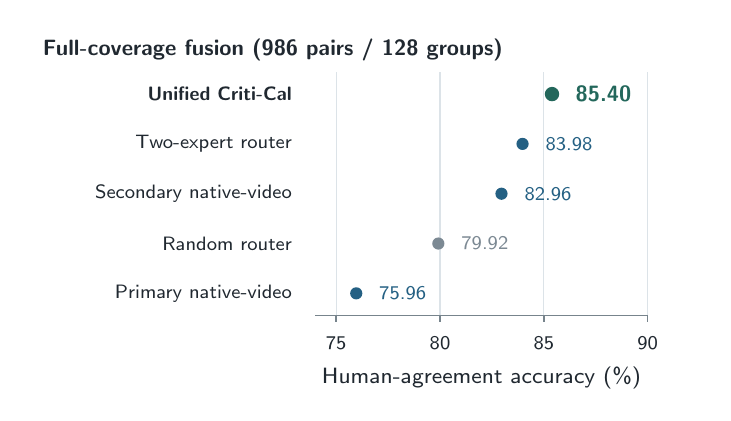
\begin{tikzpicture}[
  x=1pt,y=1pt,
  evlabel/.style={anchor=east,font=\sffamily\fontsize{7.5}{9}\selectfont,text=evInk},
  evtick/.style={anchor=north,font=\sffamily\fontsize{7.2}{8.6}\selectfont,text=evInk},
  evval/.style={anchor=west,font=\sffamily\fontsize{7.4}{8.8}\selectfont}
]
\path[use as bounding box] (0,-24) rectangle (244,108);

% Plot area: x in [104, 224] maps accuracy [74, 90] -> x = 104 + (acc - 74) * 7.5
% y rows: 0->12, 1->30, 2->48, 3->66, 4->84
\foreach \acc/\xpos in {75/111.5, 80/149.0, 85/186.5, 90/224.0} {
  \draw[evGrid,line width=0.5pt] (\xpos,4) -- (\xpos,92);
  \draw[evAxis,line width=0.6pt] (\xpos,4) -- (\xpos,1.5);
  \node[evtick] at (\xpos,0) {\acc};
}
\draw[evAxis,line width=0.6pt] (104,4) -- (224,4);
\node[anchor=north,font=\sffamily\fontsize{7.8}{9.2}\selectfont,text=evInk] at (164,-11)
  {Human-agreement accuracy (\%)};

% Row 0: Primary native-video (75.96%) -> x = 118.73
\node[evlabel] at (99,12) {Primary native-video};
\fill[evBlue] (118.73,12) circle (2.2pt);
\node[evval,text=evBlue] at (123.5,12) {75.96};

% Row 1: Random router (79.92%) -> x = 148.39
\node[evlabel] at (99,30) {Random router};
\fill[evGrey] (148.39,30) circle (2.2pt);
\node[evval,text=evGrey] at (153.2,30) {79.92};

% Row 2: Secondary native-video (82.96%) -> x = 171.21
\node[evlabel] at (99,48) {Secondary native-video};
\fill[evBlue] (171.21,48) circle (2.2pt);
\node[evval,text=evBlue] at (176.0,48) {82.96};

% Row 3: Two-expert router (83.98%) -> x = 178.82
\node[evlabel] at (99,66) {Two-expert router};
\fill[evBlue] (178.82,66) circle (2.2pt);
\node[evval,text=evBlue] at (183.6,66) {83.98};

% Row 4: Unified Criti-Cal (85.40%) -> x = 189.47
\node[evlabel,font=\sffamily\fontsize{7.5}{9}\selectfont\bfseries] at (99,84) {Unified \textsc{Criti-Cal}};
\fill[evTeal] (189.47,84) circle (2.6pt);
\node[evval,text=evTeal,font=\sffamily\fontsize{7.6}{9}\selectfont\bfseries] at (194.5,84) {85.40};

\node[anchor=west,font=\sffamily\fontsize{8.2}{9.6}\selectfont\bfseries,text=evInk] at (2,100)
  {Full-coverage fusion (986 pairs / 128 groups)};
\end{tikzpicture}%
}
\endgroup
